\documentclass[../AnalisiDeiRequisiti.tex]{subfiles}
\begin{document}
	\section{Hex}
		\subsection{Il gioco}
			Hex è un gioco da tavolo inventato dal matematico danese Piet Hein nel 1942 e reinventato
			indipendentemente dal premio Nobel per l'economia statunitense John Nash nel
			1948.\footnote[1]{Martin Gardner, Hexaflexagons and Other Mathematical Diversions: The First
			Scientific American Book of Puzzles and Games, University of Chicago Press, 1988, p. 75,
			ISBN 978-0-226-28254-1.}\\
			In una scacchiera romboidale con caselle esagonali, due giocatori devono disporre le proprie
			pedine in modo da formare una linea continua tra i due lati opposti del proprio colore.
			Ogni giocatore ha due lati del rombo non contigui.\\
			La scacchiera può essere di dimensione 10x10, 11x11 o 14x14.\\
			I giocatori hanno due colori, solitamente rosso e blu. Alternatamente pongono una pedina in
			una casella esagonale della scacchiera.
			\begin{figure} [h!]
				\centering
				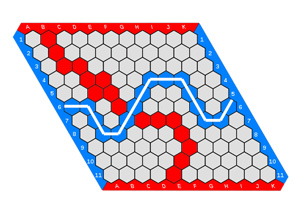
\includegraphics{./Figures/HexBoard.jpg}
				\caption{Una partita a Hex}\label{fig:1}
			\end{figure}
		\subsection{Specifiche}
			Nel Capitolato d'appalto il Proponente desidera che venga sviluppata una versione di Hex
			attraverso il prodotto \progetto.\\
			A tal proposito, il gruppo \kaleidoscode\ intende creare una versione di Hex che permetta
			di giocare in modalità pvp tra due giocatori in tutte e tre le possibili tipologie di
			scacchiere. È un requisito desiderabile per il gruppo creare un piccolo menù che permetta
			di scegliere il tipo di scacchiera così come di ottenere informazioni riguardo il
			regolamento o il gioco stesso.
\end{document}
